\section{Testing the Implementation}

To test the implementation of the presented document scanner for faults, a variety of test images are needed. For that the sample images from the \textit{OpenCV-Document-Scanner} Project [\url{https://github.com/andrewdcampbell/OpenCV-Document-Scanner}] are used.\\
In this chapter however only the flawed images will be examined in more detail, as they better illustrate the flaws in our implementation.\\

The following parameters are used after extended testing on the test images:
\begin{enumerate}
    \item \textbf{Canny Edge Detector}:\\
    Used was a Gaussian filter with a kernel of size 7x7 and a Canny Edge Detector Algorithm with a minimum threshold of 0 and a maximum threshold of 84.
    \item \textbf{Ramer–Douglas–Peucker algorithm}:\\
    Used was an accuracy parameter {\large $\bm{\epsilon}$} of 5 percent.
    \item \textbf{Adaptive Thresholding}:\\
    Used was a Gaussian filter with a kernel of size 5x5 to smooth the image. For the adaptive threshold technique a Gaussian Kernel of size $11 \times 11$ and a constant \textbf{C} of 2 were used.
\end{enumerate}

At the end of the test procedure one of the images which still got transformed incorrectly was the image \textit{notepad.jpg} from the \textit{OpenCV-Document-Scanner} Project seen in figure \ref{fig:note_error}.

\begin{figure}[H]
     \centering
     \captionsetup{justification=centering}
     \begin{subfigure}[t]{0.3\textwidth}
         \centering
         
\includegraphics[width=\textwidth]{images/4_image/notepad.png}
         \caption{Original image}
         \label{fig:note_og}
     \end{subfigure}
     \hfill
     \begin{subfigure}[t]{0.3\textwidth}
         \centering
         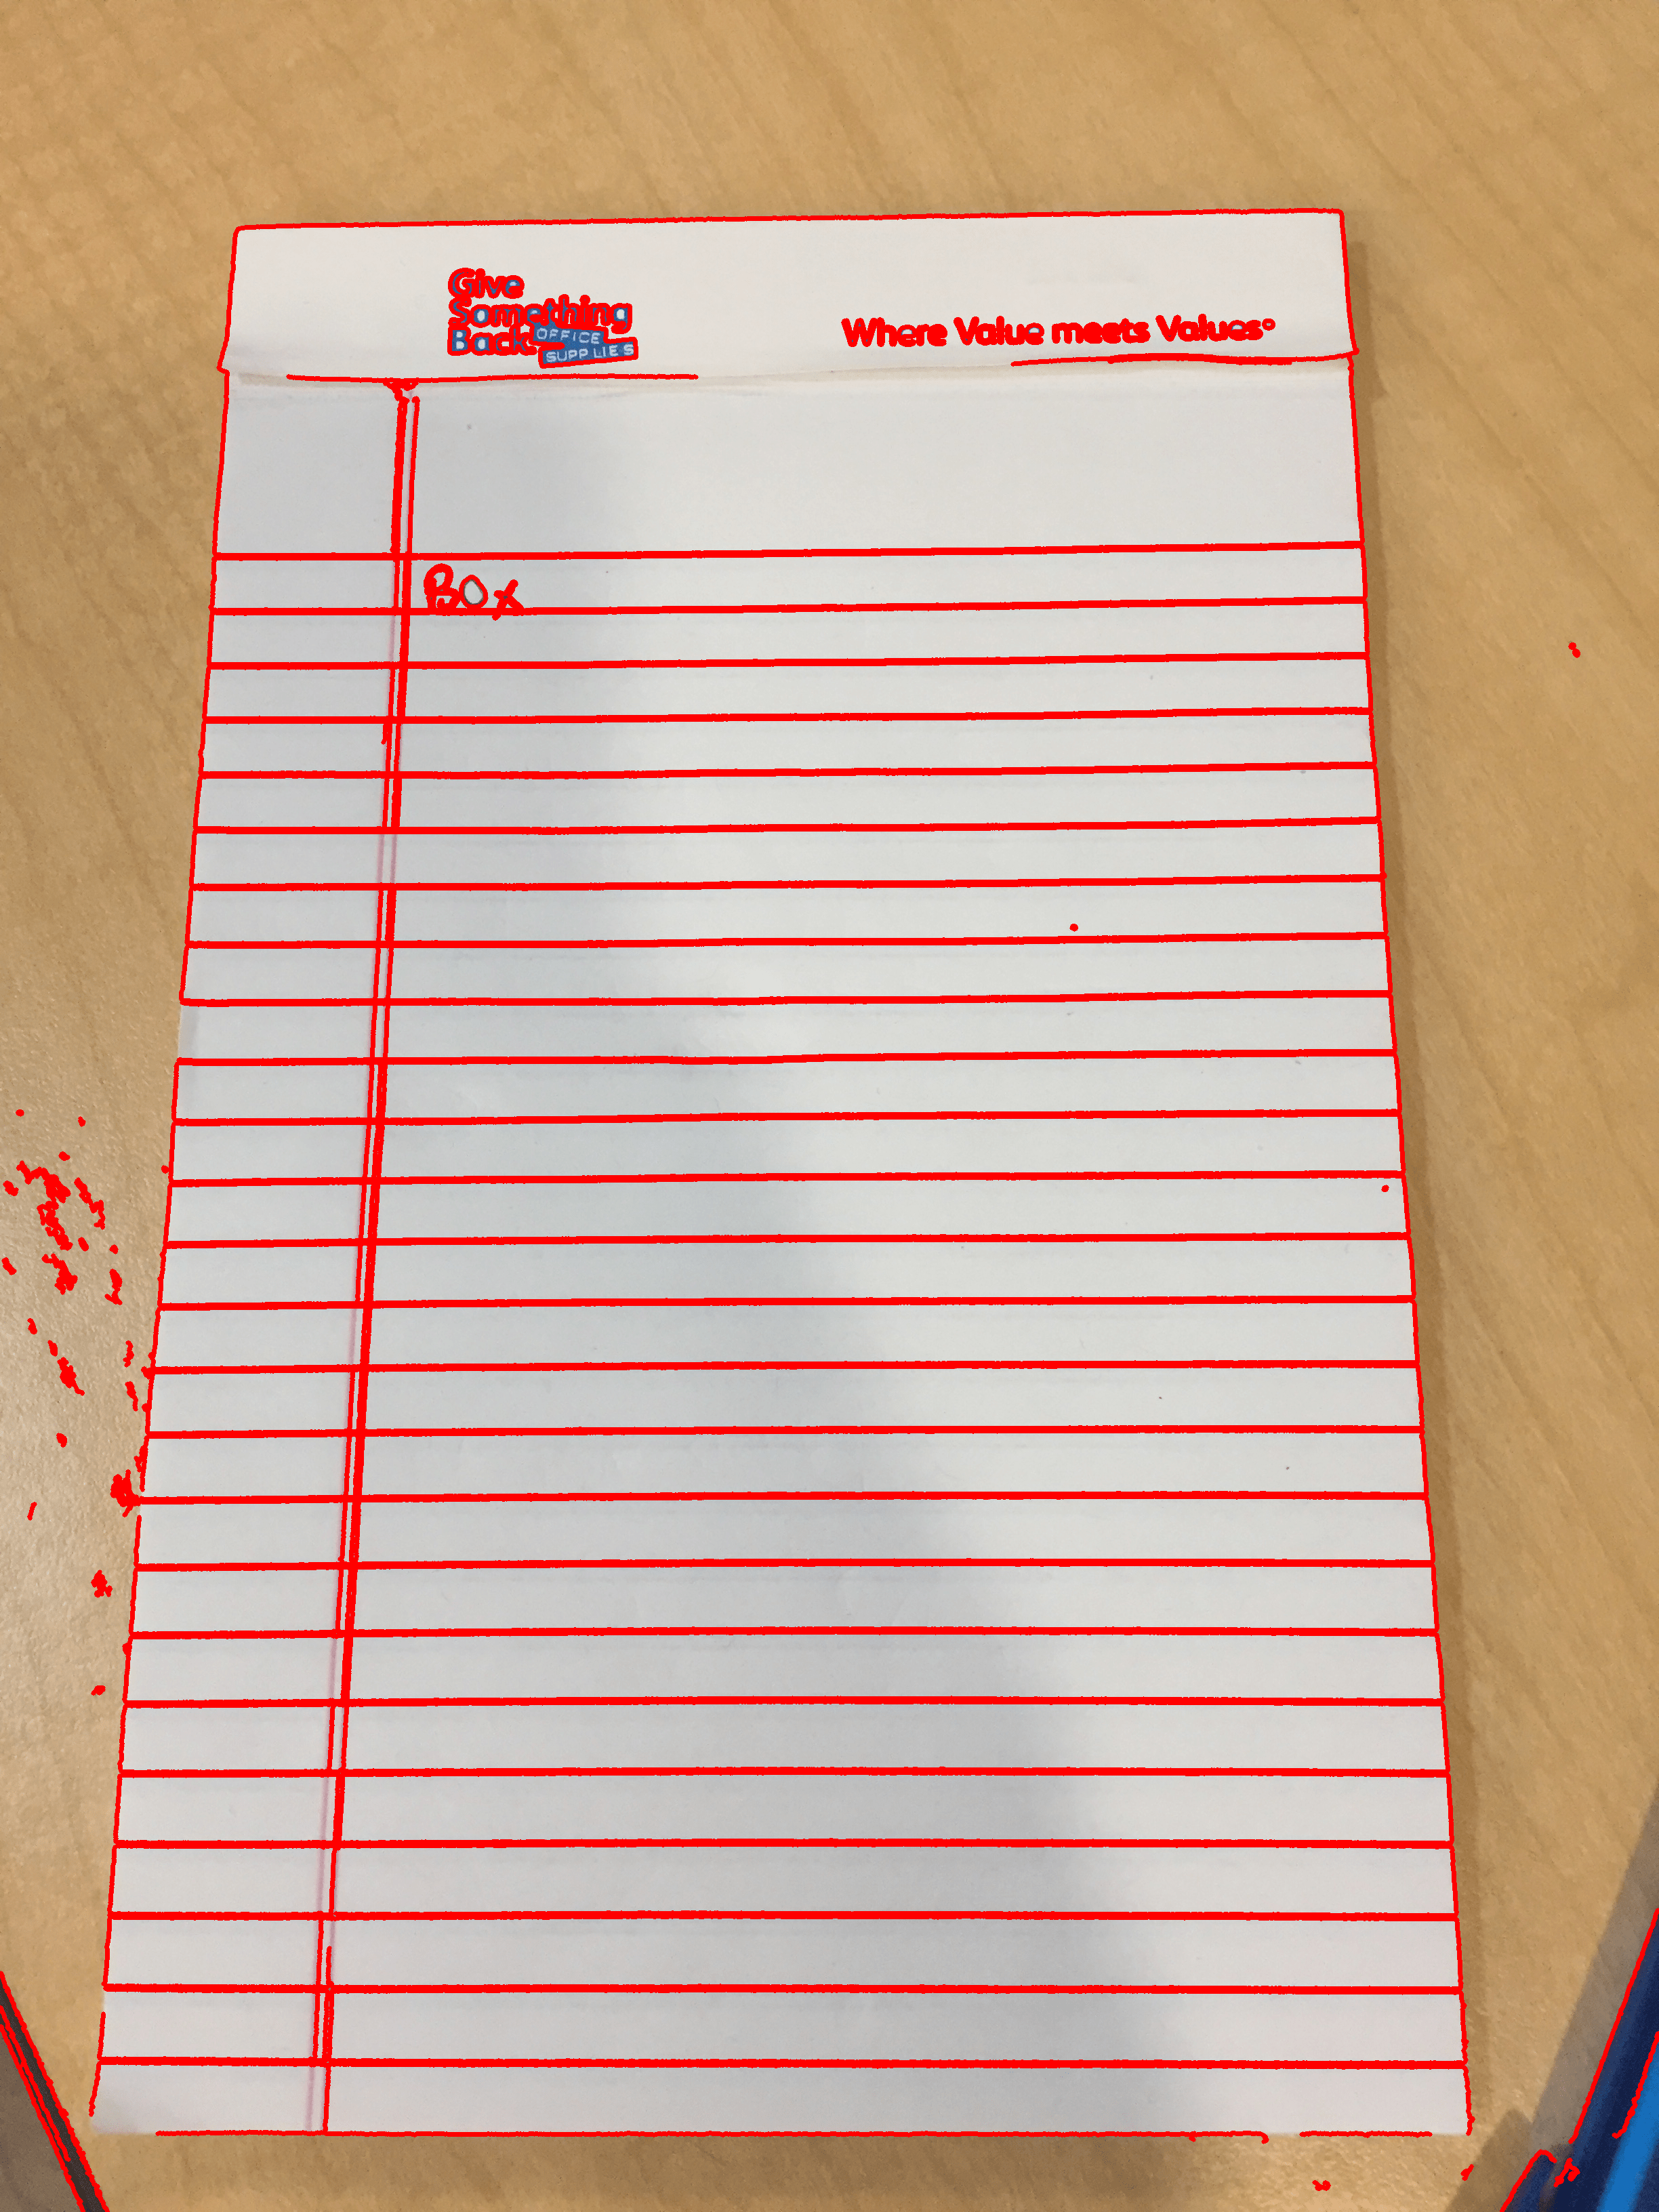
\includegraphics[width=\textwidth]{images/4_image/contours.png}
         \caption{All contours found in image}
         \label{fig:note_all}
     \end{subfigure}
     \hfill
     \begin{subfigure}[t]{0.3\textwidth}
         \centering
         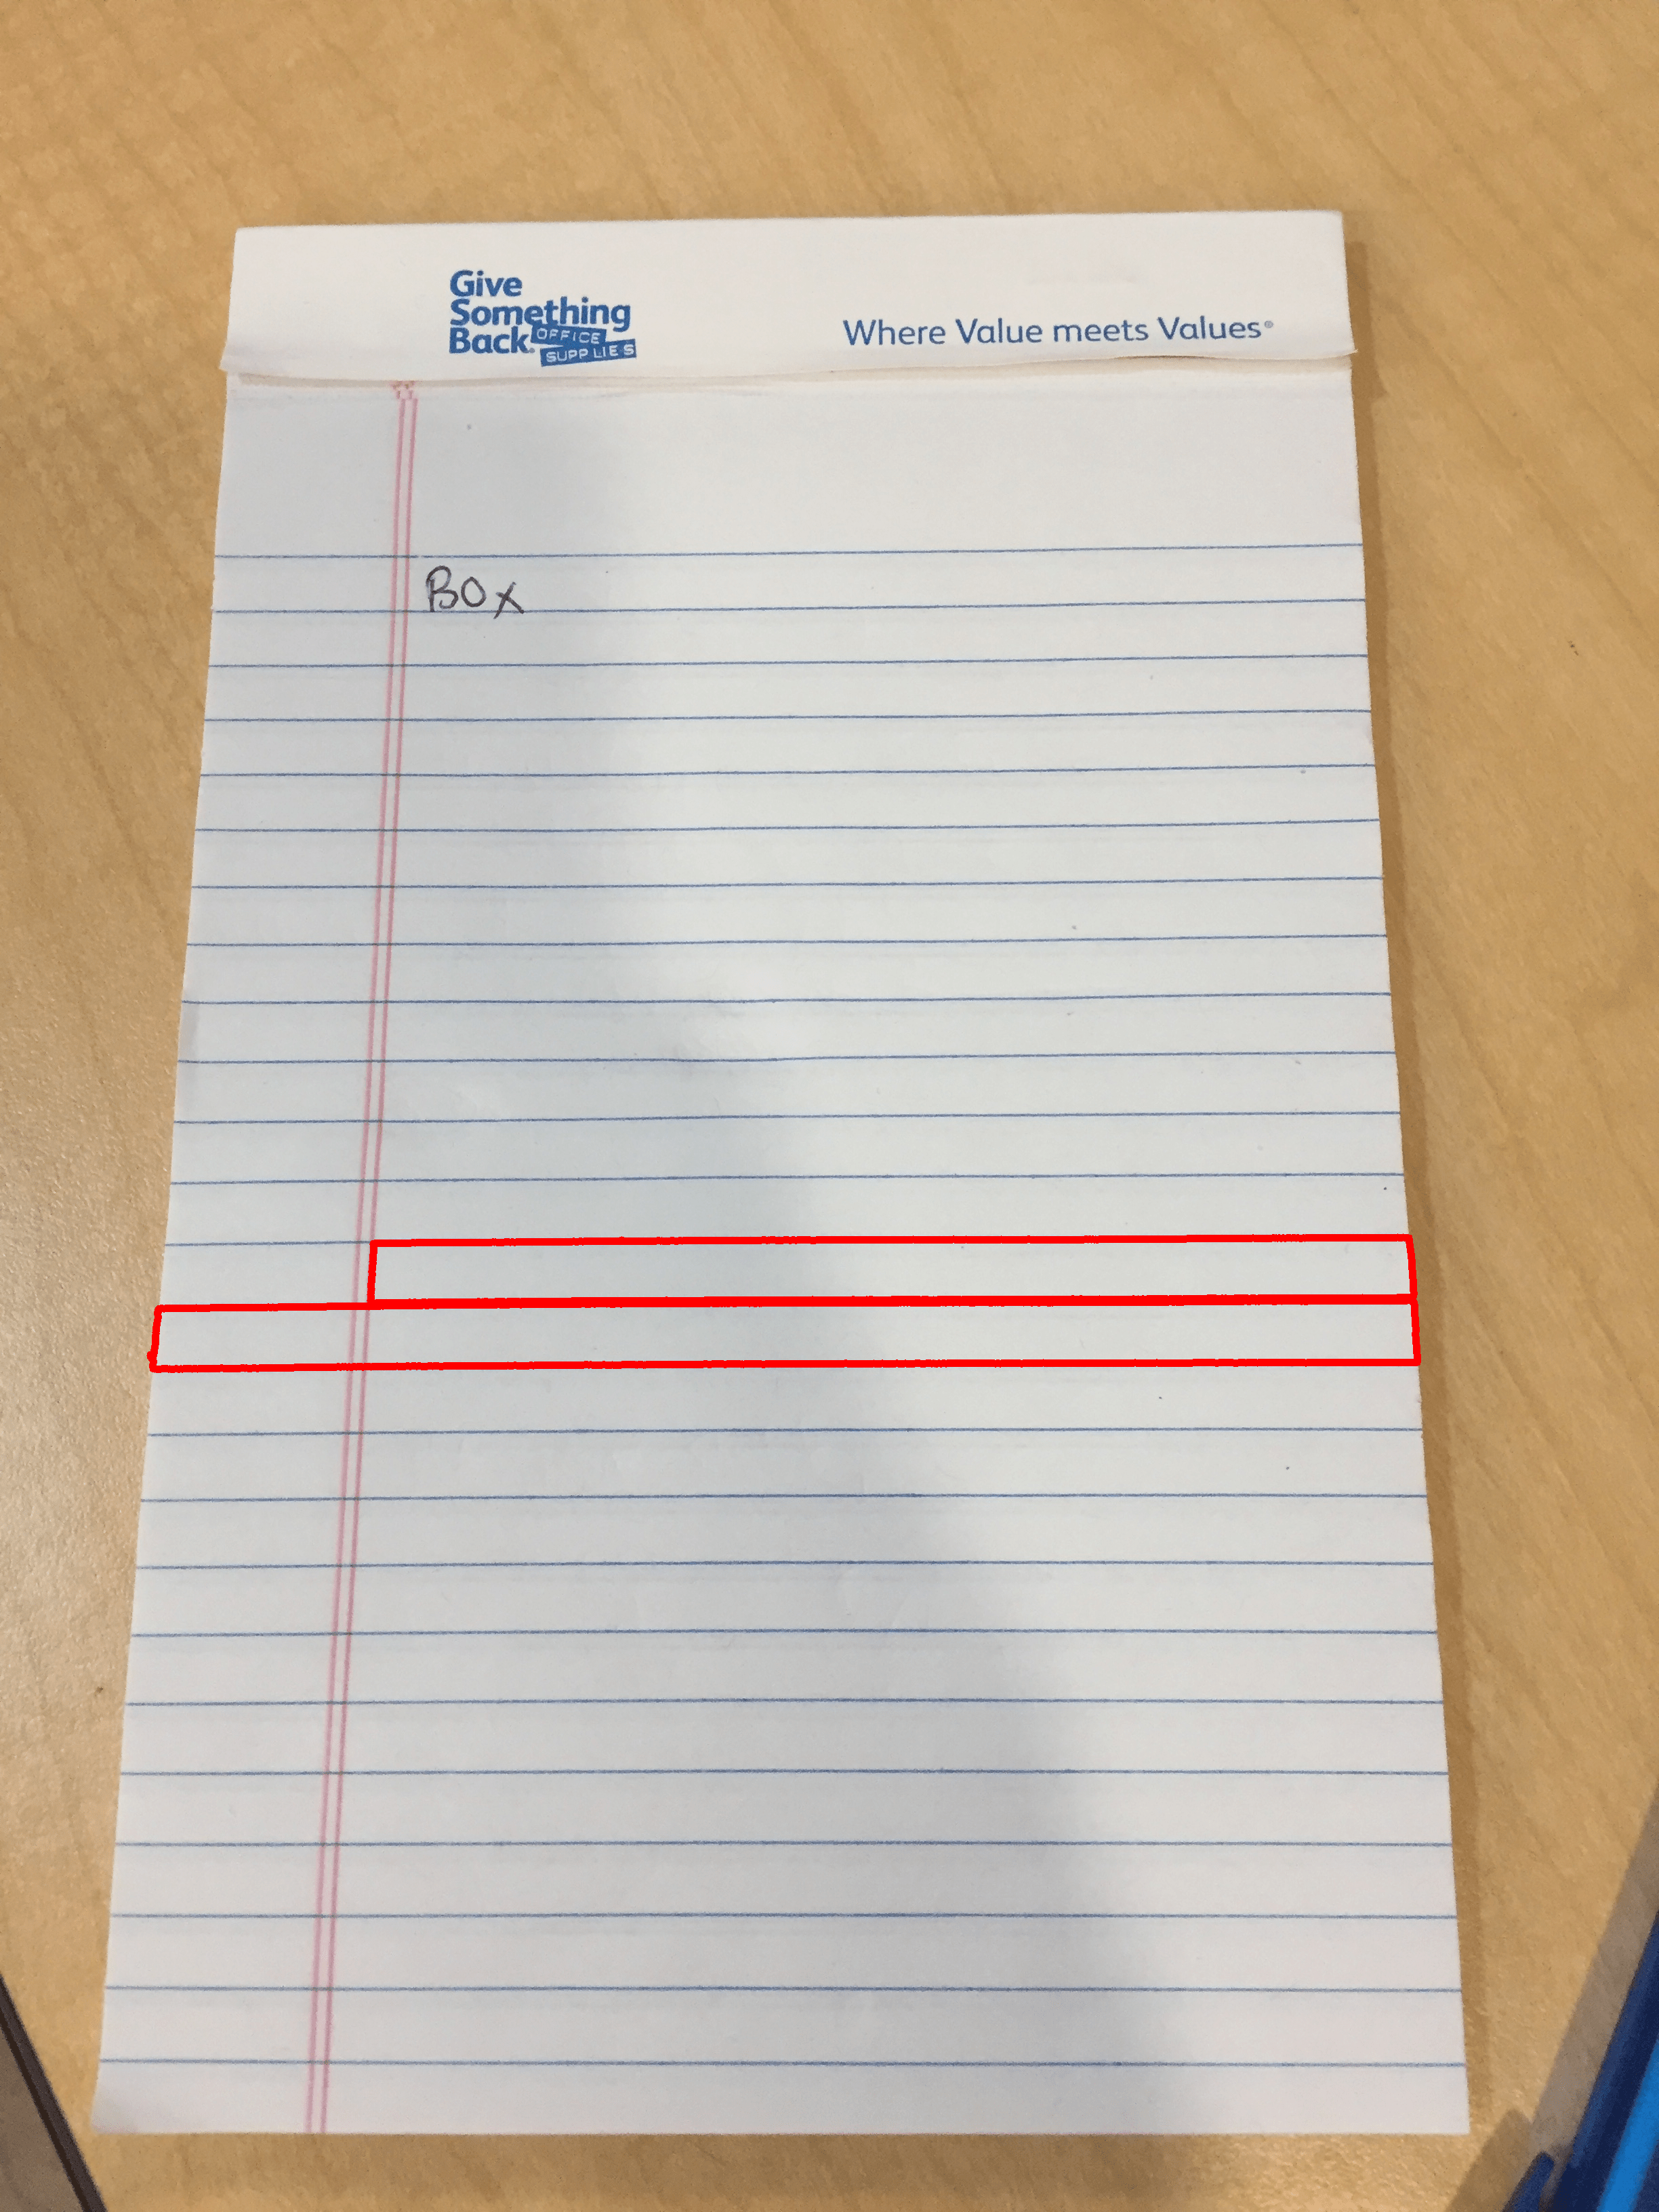
\includegraphics[width=\textwidth]{images/4_image/biggest_contour.png}
         \caption{Biggest found contour in image}
         \label{fig:note_biggest}
     \end{subfigure}
        \caption{Incorrectly transformed image of a document}
        \label{fig:note_error}
\end{figure}

\newpage

In figure \ref{fig:note_biggest} the problem can be seen clearly: The longest contour found from all possible contours is not the document edge. The problem occurs because the document edges are connected to contours inside the document, which artificially creates a longer contour that does not have to include all document corner points.\\

This is a weak point of this implementation. If there is a document that contains elements within the document which intersect the document edge, there is a chance that the longest found contour is not the document edge. Therefore the document corner points cannot be determined correctly.\\

A solution to this problem would be to let the user manually decide where to place the corner points if he is unsatisfied with the results. This could be for example if he feels that the corner points are not placed exactly on the corners of the document or if even no corner points have been detected. This is the same approach as the \textit{OpenCV-Document-Scanner} Project uses.
